\maketitle
\tableofcontents

\vspace{0.5cm}


\section{Lösungsidee}\label{sec:losungsidee}
Das Problem der Aufgabenstellung beschreibt eine Variante des NP-vollständigen Traveling-Salesman Problems.
Es ist somit nicht möglich optimale Lösungen in polynomieller Zeit für beliebige Graphen zu finden.
Für die Graphen aus den Beispieldateien ist dies aufgrund ihrer Grö{\ss}e auch nicht möglich.
Folglich müssen zur Bewältigung der Aufgabe Heuristiken herangezogen werden. \\
Zunächst wird eine initiale Lösung mittels der Nearest-Neighbour Heuristik ermittelt.
Diese wird danach iterativ durch die TwoOpt-Postoptimierung verbessert.

\subsection{Nearest-Neighbour Heuristik}\label{subsec:nearest-neighbour-heuristik}
Die Eröffnungsheuristik ist vergleichsweise einfach.
Es wird ausgehend eines Startknotens der Knoten gewählt, der die
geringste Distanz zum aktuellen Knoten hat und der noch nicht besucht wurde.
Anschlie{\ss}end wird der aktuelle Knoten zum Startknoten.
Dieses Verfahren wird so lange wiederholt, bis alle Knoten besucht wurden.

1.
Zunächst wird ein Startknoten \textit{v}\textsubscript{Start} ermittelt.
Ausgehend von \textit{v}\textsubscript{Start}, wird der Knoten \textit{v}\textsubscript{0} mit der geringsten Distanz gewählt.
\textit{v}\textsubscript{Start} und \textit{v}\textsubscript{0} werden als besucht markiert.
Die Kante \textit{e} zwischen diesen beiden Knoten wird für die Suche des nächsten Knotens genutzt.

2.
Solange es noch unbesuchte Knoten gibt, wird folgendes Verfahren wiederholt:
Betrachte in aufsteigender Distanz zu \textit{v}\textsubscript{0} alle Knoten.
Wenn die Kante, die den aktuell betrachteten Knoten und \textit{v}\textsubscript{0} verbindet, \textit{e}
derart schneidet, dass die Winkelbedingung erfüllt ist, dann wähle diesen Knoten als nächsten \textit{v}\textsubscript{0}.
Markiere \textit{v}\textsubscript{0} als besucht. \\
Sollte kein solcher Knoten ermittelt werden können, gehe einen Schritt zurück und wähle den nächst-besten Knoten (Backtracking).

\subsection{TwoOpt Postoptimierung}\label{subsec:twoopt-postoptimierung}
Zugrundelegende Idee der Optimierung ist die Dreiecksungleichung.
Diese besagt, dass eine Dreiecksseite höchstens so lang wie die Summe der beiden anderen Seiten ist.
Höchstens ist dabei der Spezialfall, dass es sich um eine Gerade handelt.
Konkret lässt sich daraus folgern, dass ein direkter Weg immer kürzer ist als über einen Umweg.
Diese Eigenschaft wird sich in der Aufgabe zunutze gemacht, indem versucht wird die Reihenfolge der besuchten Knoten eines
bereits gegeben Pfades derart zu Verändern, dass Überkreuzung reduziert werden.
\begin{figure}[h]
    \centering
    \begin{minipage}[b]{0.3\textwidth}
        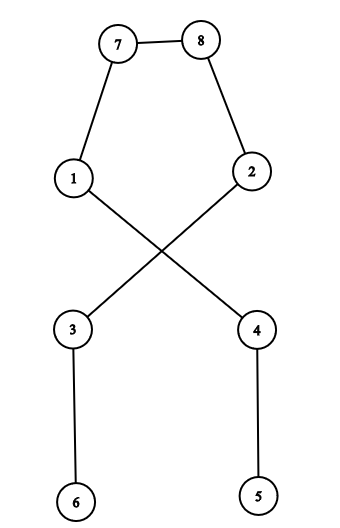
\includegraphics[width=\textwidth]{2opt1}
    \end{minipage}
    \hfill
    \begin{minipage}[b]{0.26\textwidth}
        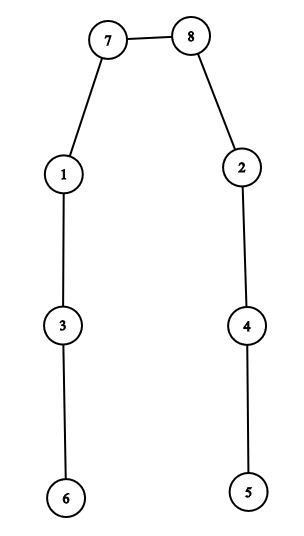
\includegraphics[width=\textwidth]{2opt2}
    \end{minipage}\label{fig:2opt}
\end{figure}
Die linke Graphik zeigt eine überkreuzte Tour.
Die Kante 1--4 schneidet die Kante 3--2 im Punkt $P$.
In der linken Abbildung werden je zwei Seiten der Dreiecke $\triangle{3P1}$ und $\triangle{42P}$ passiert.
Dies kann unter berücksichtigung der Dreiecksungleichung optimiert werden, indem jeweils nur eine der Seiten traversiert wird.
Die rechte Graphik zeigt wie die Tour dafür verändert werden muss.
Die ursprüngliche Reihenfolge 6--3--2--8--7--1--4--5 wird zu 6--3--1--7--8--2--4--5.
Durch beibehalten der Knoten und Umkehrung der Reihenfolge einer Teilroute,
im Beispiel bleibt 6--3 und 4--5 erhalten und 2--8--7--1 wird zu 1--7--8--2, kann die Strecke der Gesamttour reduziert werden. \\
Idealerweise werden alle Überkreuzungen innerhalb der Tour durch geschicktes Vertauschen entfernt.
Dieser Ansatz findet allerdings nur ein lokales Minimum bezüglich der Strecke der Gesamttour.
Möglicherweise muss zuerst eine Vertauschung vorgenommen werden, die die Gesamtstrecke erhöht, um
danach in einen besseren Zustand als zuvor zu gelangen.
Um das globale Minimum (oder wenigstens ein besonders gutes lokales Minimum) zu finden, wird der stochastische
Optimierungsalgorithmus des Simulated Annealings verwendet.

\subsection{Simulated Annealing}\label{subsec:simulated-annealing}
Der Algorithmus ist von dem natürlichen Prozess des Abschreckens von Metallen inspiriert, genannt "annealing" auf
Englisch, bei dem Metalle durch Erhitzen und langsames Abkühlen verfestigt werden.
Es wird eine simulierte Temperatur $T$ eingeführt.
Zunächst werden zwei Knoten der Tour zufällig gewählt.
Sofern dabei nicht die Winkelbedingung verletzt wird, wird die Tour errechnet, welche entstehen würde,
wenn die beiden Knoten vertauscht werden.
Das hei{\ss}t, die Teiltour, welche durch die beiden gewählten Knoten begrenzt wird, wird umgekehrt.
Ist die resultierende Tour besser als die bisherige, so werden die Knoten vertauscht.
Ist die Tour schlechter als die bisherige, so wird diese, sowohl abhängig von der
aktuellen Temperatur $T$, als auch der absoluten Änderung der Länge, sowie Abhängig eines
Zufallswertes entweder gewählt oder verworfen.
Die Anzahl der erfolgten verbessernden oder verschlechternden Vertauschungen werden gezählt.
Nach einer gewissen Zahl solcher Operationen wird $T$ abgekühlt (reduziert).
Grundsätzlich gilt, eine höhere Temperatur erlaubt ungünstige Vertauschungen wahrscheinlicher als eine niedrige Temperatur.
Diese Vorgehensweise erlaubt gro{\ss}e Schwankungen am Anfang des Verfahrens, welche sich aber im Optimalfall um ein gutes
Minimum gegen Ende einpendeln.
Ausschlaggebend für die Ergebnisqualität sind die gewählten Parameter.
Diese sind die Temperatur $T$, die Abkühlrate, die Anzahl der verbessernden Operationen bis zur Abkühlung sowie die Gesamtzahl
an Operationen bis zur Abkühlung.


\section{Umsetzung}\label{sec:umsetzung}
Die Implementierung erfolgt in Java 17. \\
Die Beispieldateien enthalten Punkte mit einer X- und Y-Koordinate.
Anhand der Punkte wird ein vollständiger, ungerichteter, gewichteter Graph erstellt.
Zur Berechnung der Kantengewichte muss die Distanz der Punkte zueinander ausgerechnet werden.
Dies erfolgt, indem die Ortsvektoren der einzelnen Punkte gebildet werden, diese voneinander abgezogen werden, um die
Verbindungsvektoren zu erhalten und anschlie{\ss}end den Betrag dieser zu errechnen.
\begin{lstlisting}[label={lst:distance}]
private Double length(Point a, Point b) {
    return Math.sqrt((a.x() - b.x()) * (a.x() - b.x()) + (a.y() - b.y()) * (a.y() - b.y()));
}
\end{lstlisting}
Um den ``Abbiege-Winkel'' an einem Knoten auszurechnen, wird der Schnittwinkel der beiden Richtungsvektoren der
betrachteten anliegenden Kanten ausgerechnet.
Ist dieser mindestens 90° gro{\ss}, so ist die Winkelbedingung erfüllt.
\begin{lstlisting}[label={lst:vector-calc}]
public static boolean matchesAngleCriteria(Vector first, Vector second) {
    double degree = VectorCalculator.calcDegree(first, second);
    return degree >= 90;
}

public static Double calcDegree(Vector a, Vector b) {
    double dotProduct = a.x() * b.x() + a.y() * b.y();
    double lengthA = length(a);
    double lengthB = length(b);
    return Math.toDegrees(Math.acos(dotProduct / (lengthA * lengthB)));
}

public static Double length(Vector vector) {
    return Math.sqrt(vector.x() * vector.x() + vector.y() * vector.y());
}
\end{lstlisting}

\subsection{Simulated Annealing}\label{subsec:simulated-annealing-implementation}
Wie bereits beschrieben, hängt die Entscheidung, ob eine Vertauschung im betrachteten Pfad von verschiedenen Parametern ab.
Konkret wird ein Zug welcher die Gesamtlänge der Tour um $d$ erhöht genau dann erlaubt,
wenn $\mathrm{e}^{-d/T}$ grö{\ss}er ist als ein Zufallswert zwischen 0 und 1.
Zum Vergleich, für $T=500$ verhält sich die Funktion wie folgt:
\begin{table}[h]
    \centering
    \begin{tabular}{|l|l|l|l|l|l|l|l|}
        \hline
        X & 50    & 200   & 350   & 500   & 650   & 800   & 950   \\ \hline
        Y & 0,905 & 0,670 & 0,497 & 0,368 & 0,273 & 0,202 & 0,150 \\ \hline
    \end{tabular}
    \caption{Temperatur 500}
    \label{tab:simulated-annealing}
\end{table}
Neben der Temperatur gibt es noch weitere Parameter.
Diese beschreiben, wie und wie oft sich die Temperatur abkühlt.
Die Funktion, welche das Abkühlverhalten der Temperatur beschreibt, ist in diesem Fall linear, könnte aber auch beliebig komplex sein.
\begin{lstlisting}[label={lst:reduce-temperatur}]
private void reduceTemperatur() {
    this.temperatur = temperaturModifier * temperatur;
}
\end{lstlisting}
Die Abkühlrate liegt typischerweise zwischen $0.9$ und $0,99$.
Die letzten beiden Parameter bestimmen darüber, nach wie vielen Operationen die Temperatur abkühlt.
$a$ meint die Anzahl der verbessernden Iterationen und $b$ meint die Anzahl der Iterationen insgesamt.\\
Im Allgemeinen haben sich die Parameter $Starttemperatur = 100$ $Abk\ddot uhlrate = 0,9$ $a = 50$ $b = 100$ als gute
Konfiguration erwiesen, die vergleichsweise gute Ergebnisse für beliebige Eingabe liefert. \\
Da die Simulated Annealing Methode kein klar definiertes Ziel bzw.\ Ende besitzt wird das Verfahren über die Zeitdauer limitiert.
Um das Problem, dass es sich um ein stochastisches Verfahren handelt und damit die Qualität der Lösung schwanken kann,
zu entgehen, wird das Verfahren öfters für die gleiche Ausgangstour wiederholt.
Um die Wartezeit zu reduzieren, wird der Prozess mittels der Reactive Streams
Library\footnote{https://github.com/reactive-streams/reactive-streams-jvm} parallelisiert. \\

\subsection{Komplexitätsbetrachtung}\label{subsec:komplexitatsbetrachtung}
Eine optimale Lösung zu finden, würde bedeuten, alle Permutationen bestehend aus allen Knoten auszuprobieren.
Für den ersten Knoten gibt es $n$ Möglichkeiten, für den zweiten $n - 1$ etc.
Damit ergibt sich die Laufzeit $n!$.
Im schlechtesten Fall muss die Nearest-Neighbour Heuristik, wie oben beschrieben, auch an jedem Knoten jeden noch nicht besuchten Knoten ausprobieren.
Damit folgt für die Nearest-Neighbour Heuristik die Worst-Case-Laufzeit von $n!$.
Tatsächlich findet der Algorithmus nahezu instantan eine Lösung.
Eine Ausnahme hierbei stellt das Beispiel 5 dar.
Für genaueres siehe~\ref{subsec:beispiel-5}. \\
Um auch Beispiele wie Beispiel 5 lösen zu können, werden für jeden Knoten des Graphens die Anzahl der möglichen
Vorgänger- und Nachfolgerkanten ermittelt, um diese im Zweifelsfall in die Auswahl des nächsten Knotens
in der Nearest Neighbour Heuristik einflie{\ss}en zu lassen.
Das hat eine Laufzeit von $n^2$ \\
Die Postoptimierung vertauscht Knoten in einer linearen Laufzeit.
Die Laufzeit der 2opt-Optimierung ist unabhängig von der Grö{\ss}e des Graphens, lediglich die Parameter entscheiden über die
Anzahl der Operationen.

\subsection{Kann das Programm immer eine Lösung finden?}\label{subsec:losbarkeit}
Bevor nach einer Route gesucht wird, werden alle Knoten dahingehend geprüft, ob es mindestens eine valide Kombination
an anliegenden Kanten gibt, über welche der Knoten traversiert werden kann.
Es darf maximal zwei Knoten geben, die diese Eigenschaft nicht besitzen.
Diese zwei Knoten müssen Start- und Endknoten sein.
Gibt es mehr als zwei solcher Knoten, ist es nicht möglich alle diese Knoten zu erreichen, und somit auch nicht möglich
eine Lösung zu ermitteln.
Ein Beispiel für einen solchen nicht lösbaren Graphen wäre Graph in welchem
die drei äu{\ss}ersten Punkte ein gleichseitiges Dreieck bilden.


\section{Beispiele}\label{sec:beispiele}
Die Beispiele entsprechen den Beispieldateien.
Beispiel 1 bis 3 lassen sich derart gut durch die Nearest-Neighbour Heuristik lösen, dass die Postoptimierung keine Verbesserungen erzielt.
Die Graphiken zeigen jeweils wie die ermittelte Tour verläuft und wie lang diese ist.
Gegebenenfalls sind zudem auch die Parameter der Postoptimierung angegeben.
Die vollständige Programmausgabe ist im Anhang zu finden.

\subsection{Beispiel 1}\label{subsec:beispiel-1}
\begin{figure}[h]
    \centering
    \begin{minipage}[b]{0.6\textwidth}
        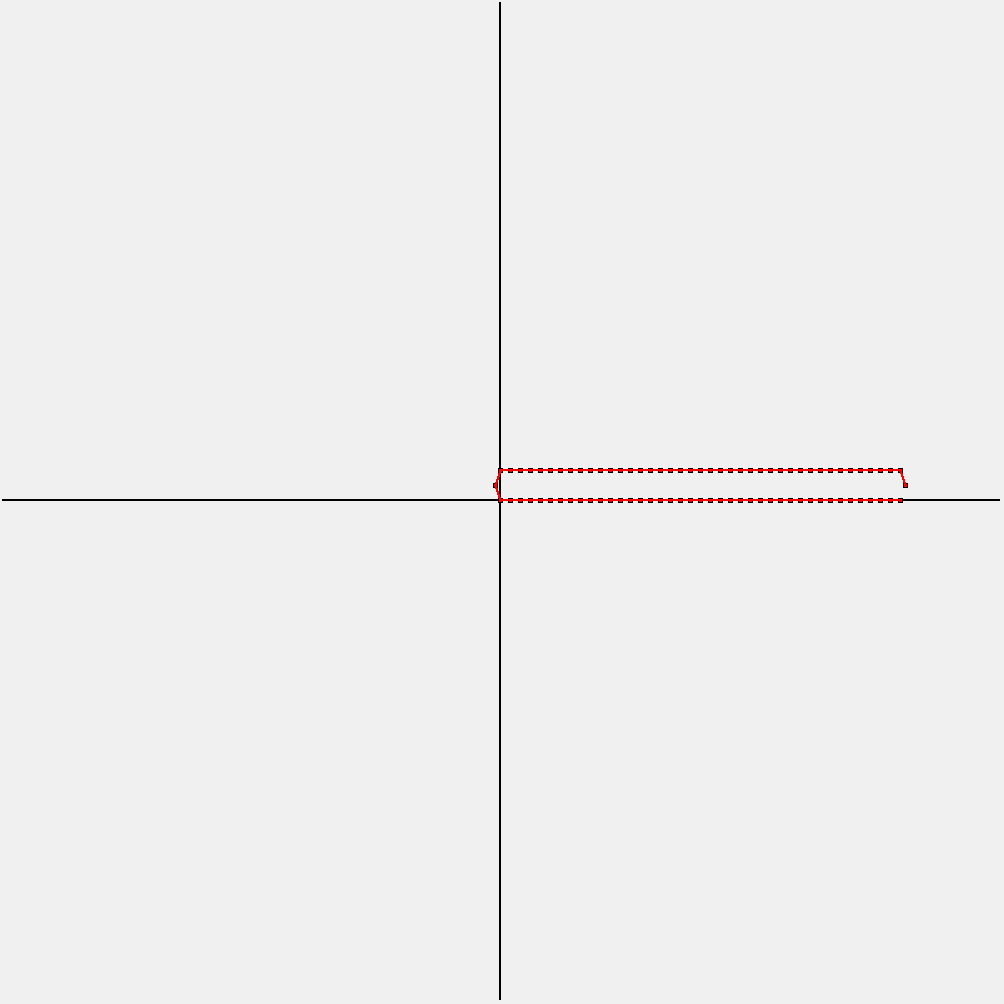
\includegraphics[width=\textwidth]{naivwenigerkrumm1}
        \caption{Naive Lösung Länge 847.4341649025257}
    \end{minipage}\label{fig:wenigerkrumm1}
\end{figure}
\FloatBarrier

\subsection{Beispiel 2}\label{subsec:beispiel-2}
\begin{figure}[h]
    \centering
    \begin{minipage}[b]{0.6\textwidth}
        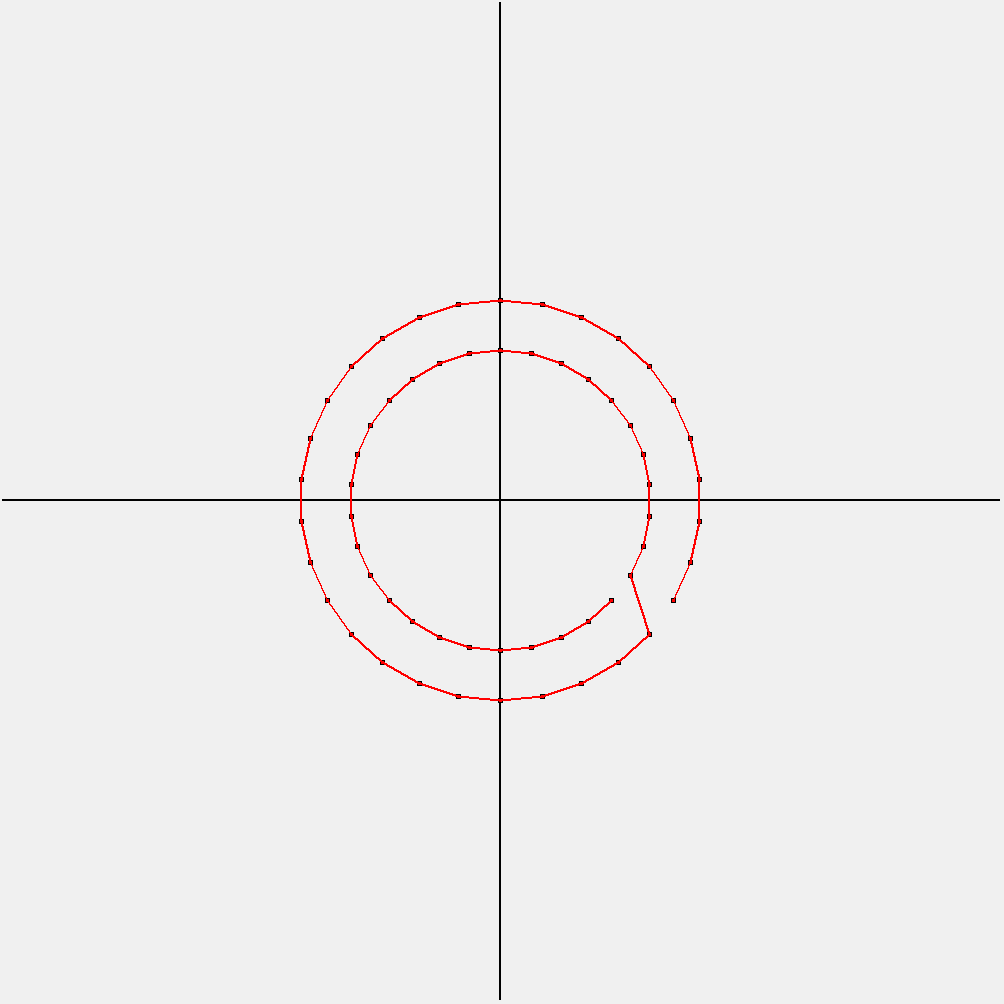
\includegraphics[width=\textwidth]{naivwenigerkrumm2}
        \caption{Naive Lösung Länge 2183.6622668054965}
    \end{minipage}\label{fig:wenigerkrumm2}
\end{figure}
\FloatBarrier

\subsection{Beispiel 3}\label{subsec:beispiel-3}
\begin{figure}[h]
    \centering
    \begin{minipage}[b]{0.6\textwidth}
        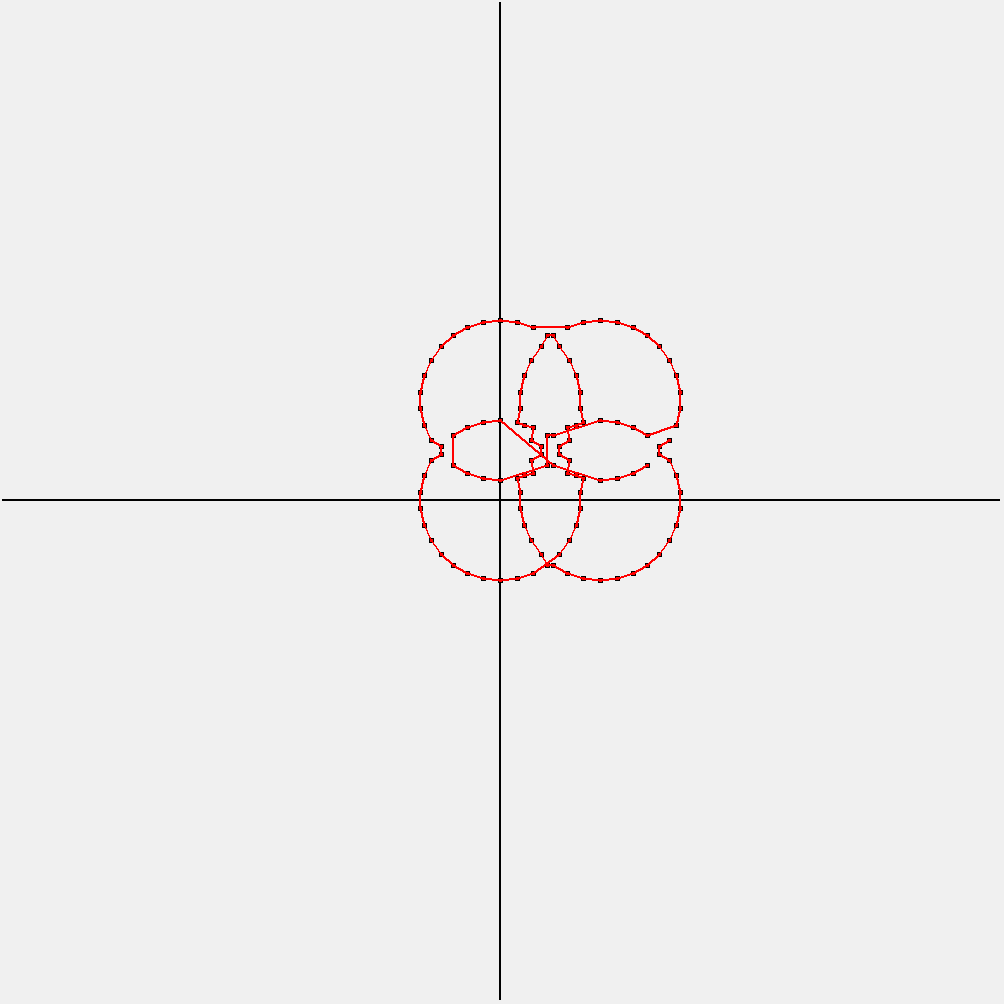
\includegraphics[width=\textwidth]{naivwenigerkrumm3}
        \caption{Naive Lösung Länge 2001.318764396512}
    \end{minipage}\label{fig:wenigerkrumm3}
\end{figure}
\FloatBarrier

\subsection{Beispiel 4}\label{subsec:beispiel-4}
\begin{figure}[h]
    \centering
    \begin{minipage}[b]{0.5\textwidth}
        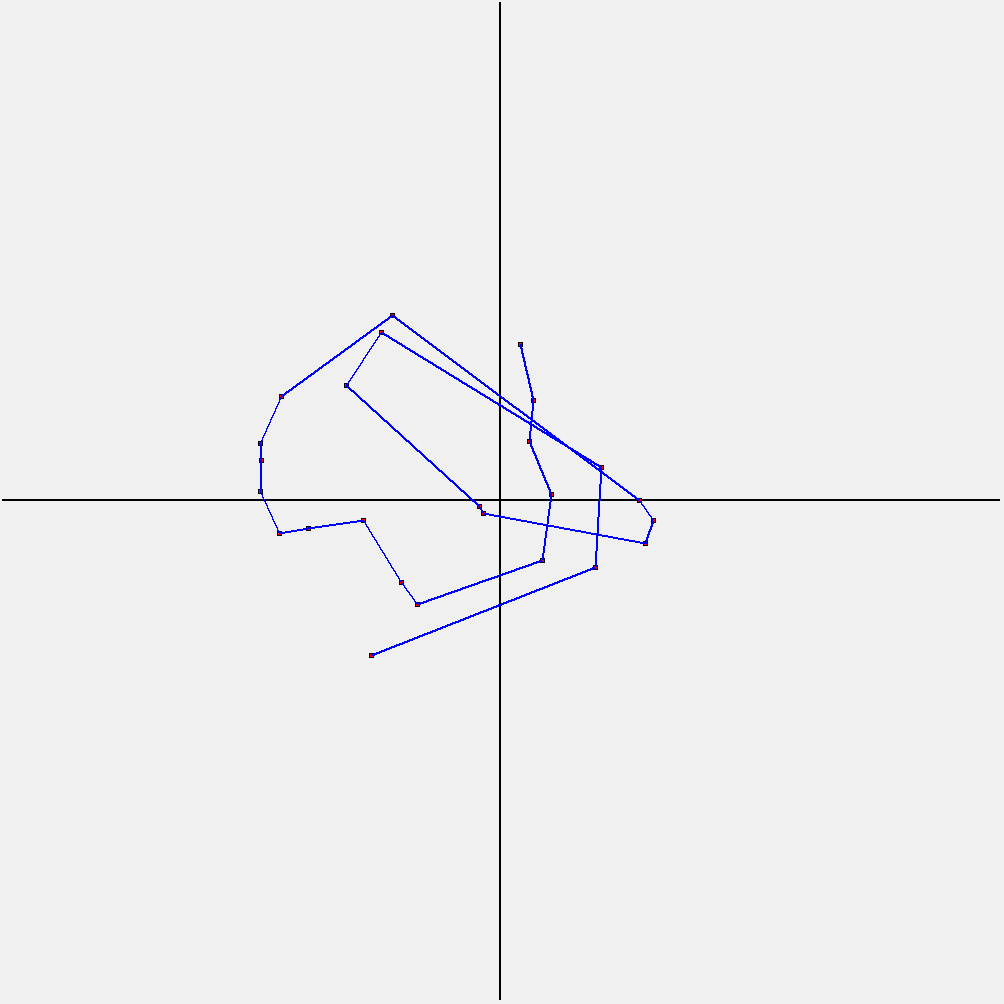
\includegraphics[width=\textwidth]{naivwenigerkrumm4}
        \caption{Naive Lösung Länge 2197.965650598992}
    \end{minipage}
    \hfill
    \begin{minipage}[b]{0.5\textwidth}
        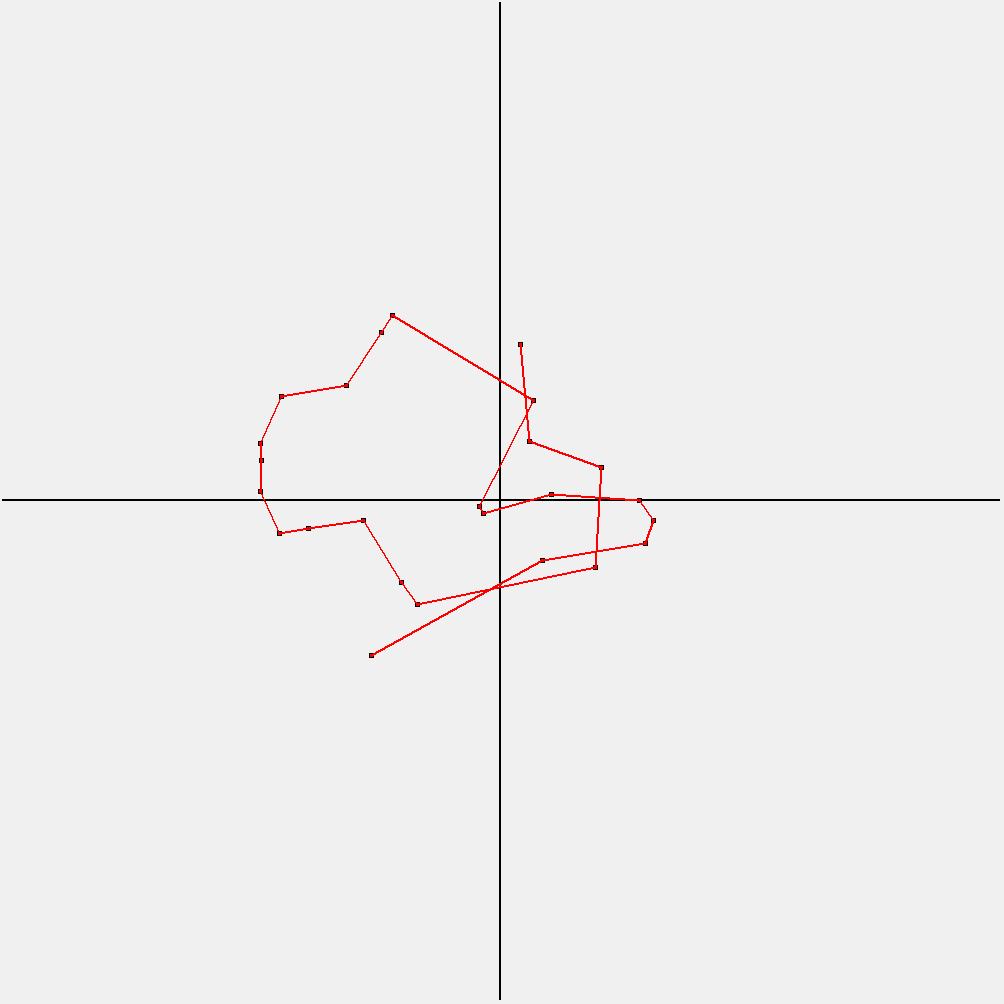
\includegraphics[width=\textwidth]{optimizedwenigerkrumm4}
        \caption{Optimierte Lösung Länge 1736.980701656645}
    \end{minipage}\label{fig:wenigerkrumm4}
\end{figure}
\begin{table}[b]
    \centering
    \begin{tabular}{|l|l|}
        \hline
        Parameter          & Wert  \\ \hline
        Starttemperatur    & 1300  \\ \hline
        Temperaturänderung & 0,985 \\ \hline
        \begin{tabular}[c]{@{}l@{}}
            Verbessernde Iterationen\\ bis zur Abkühlung
        \end{tabular}      & 10    \\ \hline
        \begin{tabular}[c]{@{}l@{}}
            Iterationen bis \\ zur Abkühlung
        \end{tabular}      & 16    \\ \hline
    \end{tabular}
    \caption{Parameterkonfiguration Beispiel 5}
    \label{tab:wenigerkrumm5}
\end{table}
\FloatBarrier

\subsection{Beispiel 5}\label{subsec:beispiel-5}
Zunächst wurde versucht mittels Nearest-Neighbour Heuristik eine initiale Lösung zu finden.
Dies führte auch nach über einer Stunde Laufzeit nicht zu einem Ergebnis.
Aufgrund dessen wurde die Nearest-Neighbour Heuristik derart modifiziert, dass nicht nur
der Abstand eines Knotens zum aktuellen Knoten in betracht gezogen wird, sondern auch
die Anzahl der möglichen Pfade die über den Knoten führen.
Je weniger solcher Pfade es gibt, desto höhere Priorität hat der Knoten in der Suche des nächsten Knotens.
Dieses Vorgehen erklärt die vergleichsweise schlechte initiale Lösung.
Um so interessanter ist es, dass die Postoptimierung dennoch zu so einem guten Ergebnis führt. \\

\begin{figure}[]
    \centering
    \begin{minipage}[b]{0.5\textwidth}
        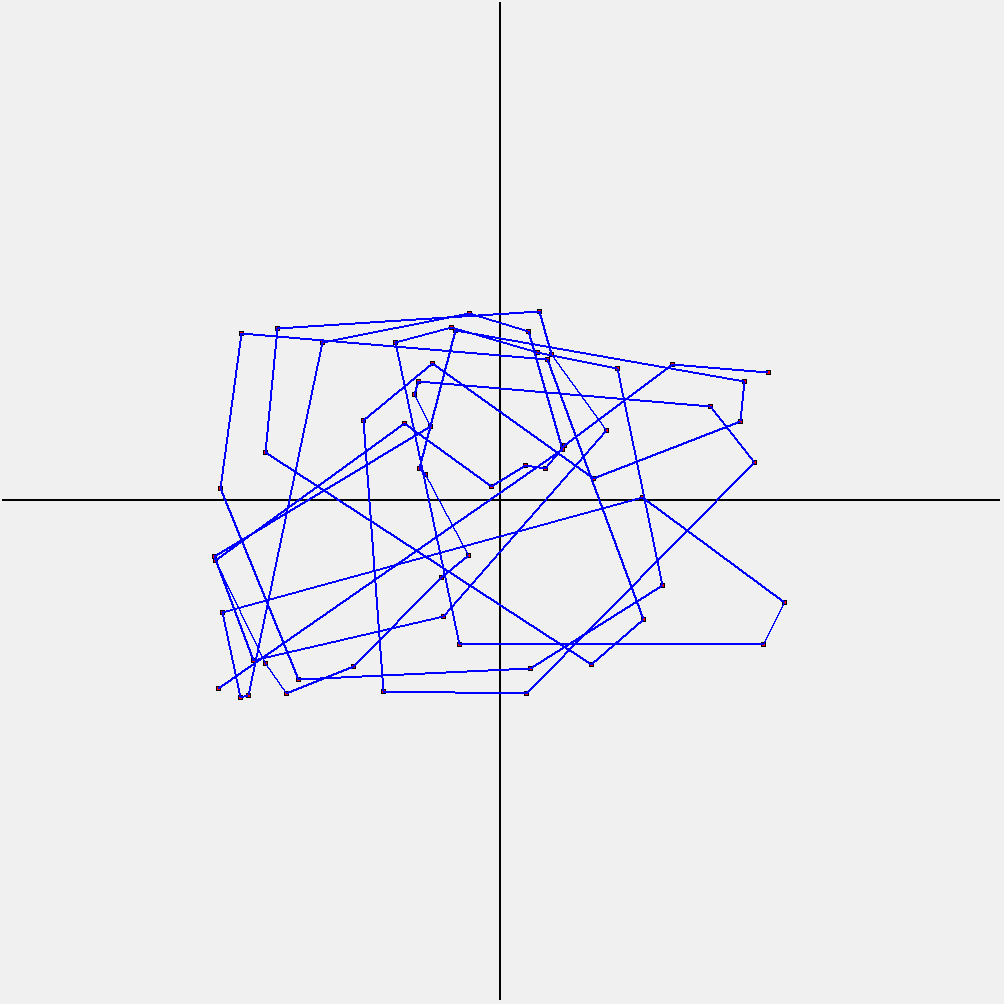
\includegraphics[width=\textwidth]{naivwenigerkrumm5}
        \caption{Naive Lösung Länge 9277.77985102936}
    \end{minipage}
    \hfill
    \begin{minipage}[b]{0.5\textwidth}
        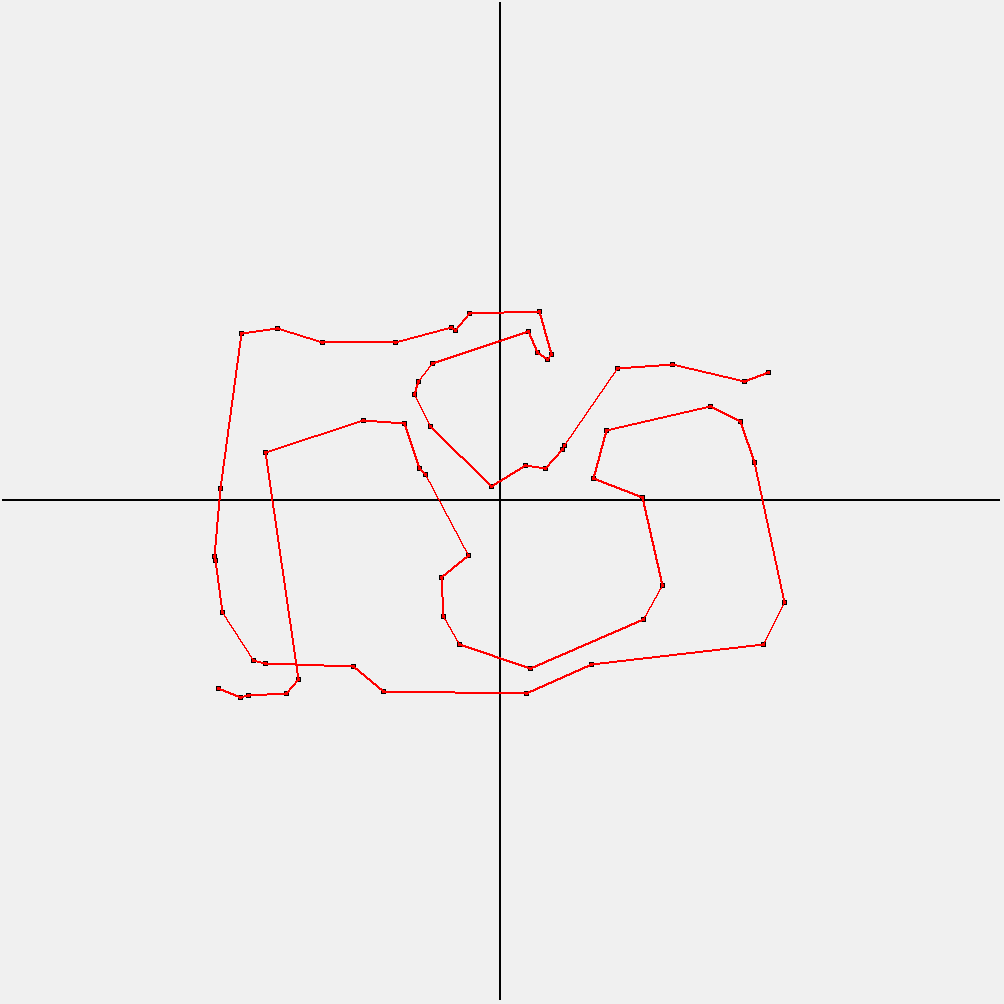
\includegraphics[width=\textwidth]{optimizedwenigerkrumm5}
        \caption{Optimierte Lösung Länge 3381.157719454162}
    \end{minipage}\label{fig:wenigerkrumm5}
\end{figure}

\begin{table}[]
    \centering
    \begin{tabular}{|l|l|}
        \hline
        Parameter          & Wert  \\ \hline
        Starttemperatur    & 1300  \\ \hline
        Temperaturänderung & 0,985 \\ \hline
        \begin{tabular}[c]{@{}l@{}}
            Verbessernde Iterationen\\ bis zur Abkühlung
        \end{tabular}      & 10    \\ \hline
        \begin{tabular}[c]{@{}l@{}}
            Iterationen bis \\ zur Abkühlung
        \end{tabular}      & 16    \\ \hline
    \end{tabular}
    \caption{Parameterkonfiguration Beispiel 5}
    \label{tab:wenigerkrumm5}
\end{table}
\FloatBarrier

\subsection{Beispiel 6}\label{subsec:beispiel-6}

\begin{figure}[t]
    \centering
    \begin{minipage}[b]{0.6\textwidth}
        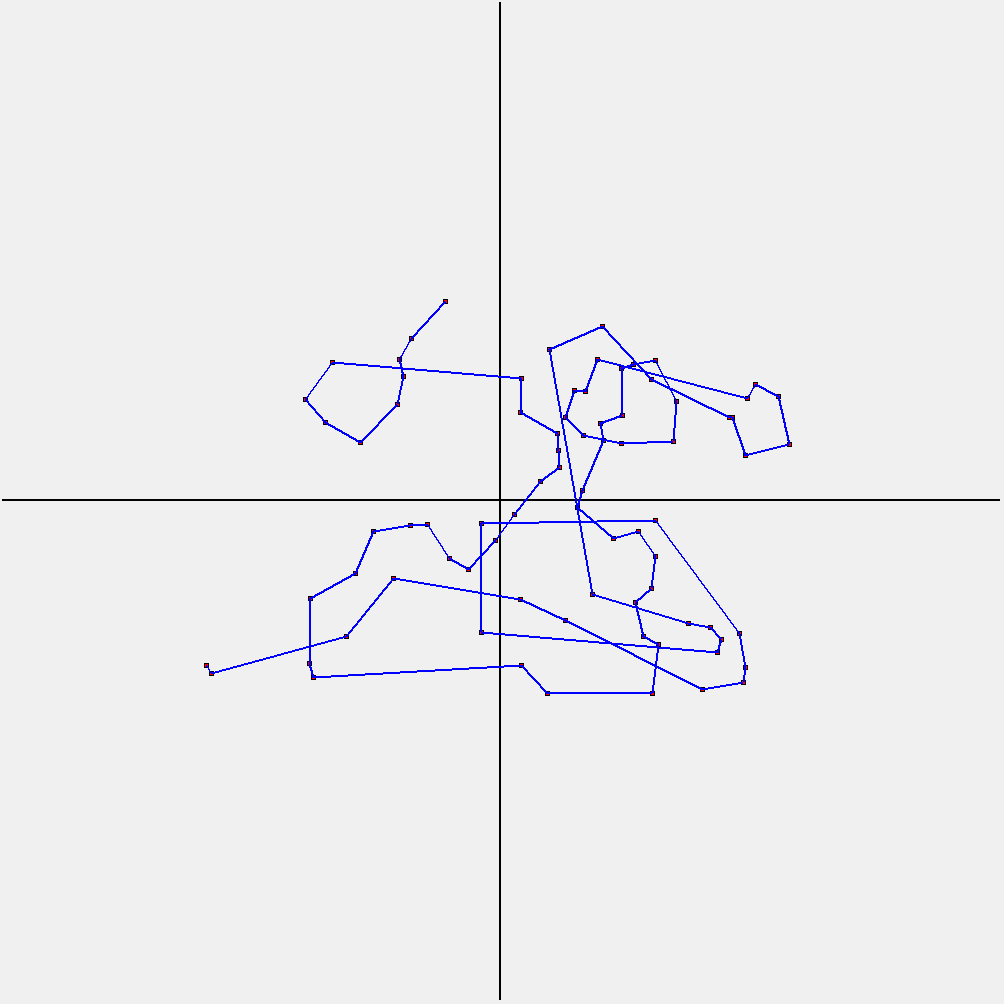
\includegraphics[width=\textwidth]{naivwenigerkrumm6}
        \caption{Naive Lösung Länge 4362.616434557695}
    \end{minipage}
    \hfill
    \begin{minipage}[b]{0.6\textwidth}
        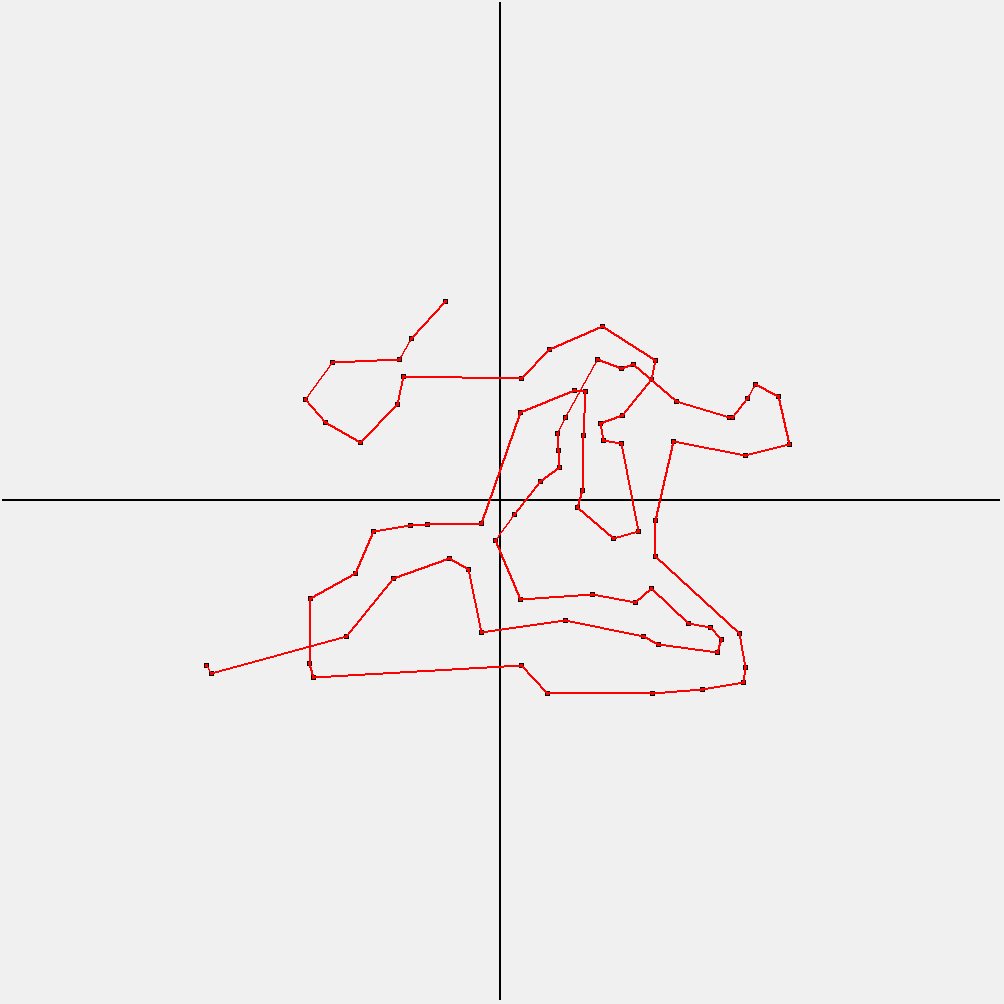
\includegraphics[width=\textwidth]{optimizedwenigerkrumm6}
        \caption{Optimierte Lösung Länge 3740.816749985773}
    \end{minipage}\label{fig:wenigerkrumm6}
\end{figure}

\begin{table}[b]
    \centering
    \begin{tabular}{|l|l|}
        \hline
        Parameter          & Wert  \\ \hline
        Starttemperatur    & 1300  \\ \hline
        Temperaturänderung & 0,985 \\ \hline
        \begin{tabular}[c]{@{}l@{}}
            Verbessernde Iterationen\\ bis zur Abkühlung
        \end{tabular}      & 10    \\ \hline
        \begin{tabular}[c]{@{}l@{}}
            Iterationen bis \\ zur Abkühlung
        \end{tabular}      & 16    \\ \hline
    \end{tabular}
    \caption{Parameterkonfiguration Beispiel 6}
    \label{tab:wenigerkrumm6}
\end{table}
\FloatBarrier

\subsection{Beispiel 7}\label{subsec:beispiel-7}

\begin{figure}[t]
    \centering
    \begin{minipage}[b]{0.5\textwidth}
        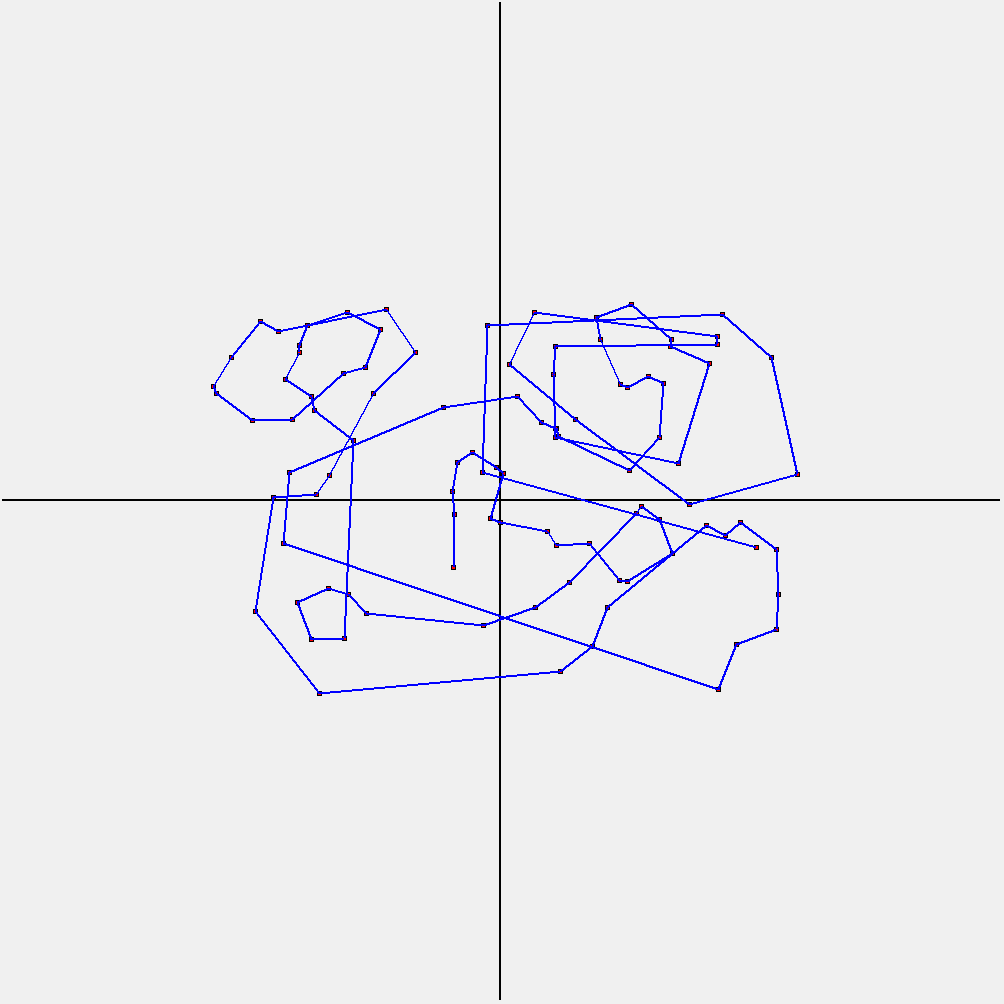
\includegraphics[width=\textwidth]{naivwenigerkrumm7}
        \caption{Naive Lösung Länge 6218.113121079488}
    \end{minipage}
    \hfill
    \begin{minipage}[b]{0.5\textwidth}
        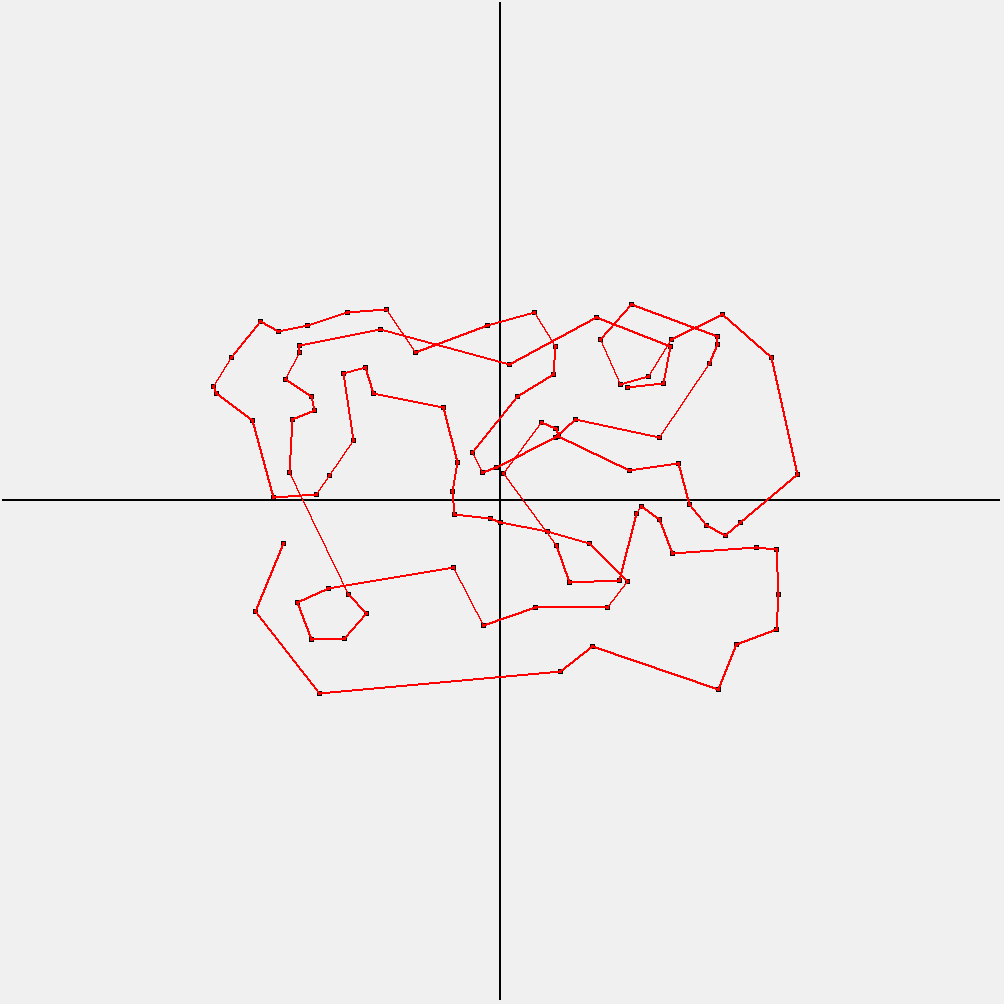
\includegraphics[width=\textwidth]{optimizedwenigerkrumm7}
        \caption{Optimierte Lösung Länge 4451.743885428826}
    \end{minipage}\label{fig:wenigerkrumm7}
\end{figure}

\begin{table}[b]
    \centering
    \begin{tabular}{|l|l|}
        \hline
        Parameter          & Wert  \\ \hline
        Starttemperatur    & 1450  \\ \hline
        Temperaturänderung & 0,975 \\ \hline
        \begin{tabular}[c]{@{}l@{}}
            Verbessernde Iterationen\\ bis zur Abkühlung
        \end{tabular}      & 10    \\ \hline
        \begin{tabular}[c]{@{}l@{}}
            Iterationen bis \\ zur Abkühlung
        \end{tabular}      & 19    \\ \hline
    \end{tabular}
    \caption{Parameterkonfiguration Beispiel 7}
    \label{tab:wenigerkrumm7}
\end{table}


\section{Quellcode}\label{sec:quellcode}
\begin{lstlisting}[label={lst:source}]
public class VectorCalculator {

    public static boolean matchesAngleCriteria(Vector first, Vector second) {
        double degree = VectorCalculator.calcDegree(first, second);
        return degree >= 90;
    }

    public static Double calcDegree(Vector a, Vector b) {
        double dotProduct = a.x() * b.x() + a.y() * b.y();
        double lengthA = length(a);
        double lengthB = length(b);
        return Math.toDegrees(Math.acos(dotProduct / (lengthA * lengthB)));
    }

    public static Double length(Vector vector) {
        return Math.sqrt(vector.x() * vector.x() + vector.y() * vector.y());
    }
}

    public ParameterConfiguration findGoodParameter(Graph graph, List<Node> path) {

        SolutionEvaluator solutionEvaluator = new SolutionEvaluator();
        System.out.println("naiv solution " + solutionEvaluator.evaluate(graph, path));
        PathPrinter pathPrinter = new PathPrinter();
        pathPrinter.print(path);
        pathPrinter.printPoints(path);
        Set<ParameterConfiguration> parameterConfigurations = this.generateAllParameterConfigurations();

        final int iterations = 5;
        final long timeLimit = 10000;

        System.out.println("iterations " + iterations);
        System.out.println("length " + parameterConfigurations.size());
        System.out.println("iterations * length " + iterations * parameterConfigurations.size());

        final int cores = Runtime.getRuntime().availableProcessors();

        System.out.println("available cores " + cores);

        double seconds = iterations * parameterConfigurations.size() * timeLimit / 1000.0;
        System.out.println("estimated time in seconds without multithreading " + seconds);
        System.out.println("estimated time in minutes without multithreading " + seconds / 60.0);
        System.out.println("estimated time in hours without multithreading " + seconds / 3600.0);

        seconds = seconds / cores;

        System.out.println("estimated time in seconds using multithreading " + seconds);
        System.out.println("estimated time in minutes using multithreading " + seconds / 60.0);
        System.out.println("estimated time in hours using multithreading " + seconds / 3600.0);


        final Map<ParameterConfiguration, ParameterTestResult> results = Flux.fromIterable(parameterConfigurations)
                .parallel()
                .flatMap(parameterConfiguration -> Mono.fromCallable(() -> {
                    // System.out.println("now testing " + parameterConfiguration);
                    ParameterTestResult result = test(parameterConfiguration, solutionEvaluator, graph, path, iterations, timeLimit);
                    // System.out.println("finished testing " + parameterConfiguration);
                    return Tuples.of(parameterConfiguration, result);
                }).subscribeOn(Schedulers.parallel()))
                .sequential()
                .collectMap(Tuple2::getT1, Tuple2::getT2)
                .block();

        String date = Instant.now().toString();

        this.saveBestResults(results, graph, date);

        return this.findBestByAverage(results, 1).stream().findAny().map(Map.Entry::getKey).orElseThrow();
    }

        @Override
    public List<Node> solve(final Graph graph, Node start) {
        traverse(graph, start);

        return solution;
    }

    @Override
    public SolvingStrategy getSolvingStrategy() {
        return SolvingStrategy.NEAREST_NEIGHBOUR_HEURISTIC;
    }


    private void traverse(Graph graph, Node start) {
        this.traverse(graph, new HashSet<>(graph.getNodes()), start, null, new ArrayList<>());
    }

    private void traverse(Graph graph, Set<Node> open, Node current, Edge last, List<Node> path) {
        if (solutionFound) {
            return;
        }
        path.add(current);
        open.remove(current);
        if (open.isEmpty()) {
            solutionFound = true;
            solution = path;
            return;
        }

        List<Edge> possibleNext = this.weightedNextEdgeProvider.calcPossibleNext(graph, current, last, open);

        for (final Edge edge : possibleNext) {
            Node next = edge.flip(current);
            traverse(graph, new HashSet<>(open), next, edge, new ArrayList<>(path));
        }
    }

public class AngleCriteriaNextEdgeProvider {

    public Set<Edge> getNext(Graph graph, Node current, Edge last) {
        final Set<Edge> set = new HashSet<>();
        for (final Edge next : graph.getNeighbouringEdges().get(current)) {
            if (last.equals(next)) {
                continue;
            }
            if (VectorCalculator.matchesAngleCriteria(last.vector(current), next.vector(current))) {
                set.add(next);
            }
        }
        return set;
    }

}


@RequiredArgsConstructor
public class WeightedNextEdgeProvider {

    private final AngleCriteriaNextEdgeProvider nextEdgeProvider;

    public List<Edge> calcPossibleNext(Graph graph, Node current, Edge last, Set<Node> open) {
        List<Edge> possibleNext;

        if (last == null) {
            possibleNext = new ArrayList<>(graph.getNeighbouringEdges().get(current));
        } else {
            possibleNext = new ArrayList<>(this.nextEdgeProvider.getNext(graph, current, last));
        }

        possibleNext.sort(Comparator.comparingDouble(Edge::weight));

        List<Edge> result = new ArrayList<>();

        for (final Edge edge : possibleNext) {
            Node next = edge.flip(current);
            if (open.contains(next)) {
                result.add(edge);
            }
        }

        return result;

    }


}


@RequiredArgsConstructor
public class NearestNeighbourHeuristic implements Solver {


    private boolean solutionFound = false;

    private List<Node> solution = null;

    private final WeightedNextEdgeProvider weightedNextEdgeProvider;

    @Override
    public List<Node> solve(final Graph graph, Node start) {
        traverse(graph, start);

        return solution;
    }

    @Override
    public SolvingStrategy getSolvingStrategy() {
        return SolvingStrategy.NEAREST_NEIGHBOUR_HEURISTIC;
    }


    private void traverse(Graph graph, Node start) {
        this.traverse(graph, new HashSet<>(graph.getNodes()), start, null, new ArrayList<>());
    }

    private void traverse(Graph graph, Set<Node> open, Node current, Edge last, List<Node> path) {
        if (solutionFound) {
            return;
        }
        path.add(current);
        open.remove(current);
        if (open.isEmpty()) {
            solutionFound = true;
            solution = path;
            return;
        }

        List<Edge> possibleNext = this.weightedNextEdgeProvider.calcPossibleNext(graph, current, last, open);

        for (final Edge edge : possibleNext) {
            Node next = edge.flip(current);
            traverse(graph, new HashSet<>(open), next, edge, new ArrayList<>(path));
        }
    }


}


/**
 * swap cities using simulated annealing to allow worsening swaps
 * this hopefully evades local minima
 */
@RequiredArgsConstructor
public class TwoOptPostOptimization implements PostOptimization {

    private final static ParameterConfiguration DEFAULT_CONFIGURATION =
            new ParameterConfiguration(100.0,
                    0.9,
                    50,
                    100);

    private final SolutionEvaluator solutionEvaluator;
    private final double temperaturModifier;
    private final int improvingIterationsUntilCooling;
    private final int iterationsUntilCooling;
    private double temperatur;


    public TwoOptPostOptimization(SolutionEvaluator solutionEvaluator) {
        this(solutionEvaluator, DEFAULT_CONFIGURATION);
    }

    public TwoOptPostOptimization(SolutionEvaluator solutionEvaluator,
                                  ParameterConfiguration configuration) {
        this.solutionEvaluator = solutionEvaluator;
        this.temperatur = configuration.startingTemperature();
        this.temperaturModifier = configuration.temperaturModifier();
        this.improvingIterationsUntilCooling = configuration.improvingIterationsUntilCooling();
        this.iterationsUntilCooling = configuration.iterationsUntilCooling();
    }

    @Override
    public List<Node> optimize(final Graph graph, final List<Node> tour, long timeLimit) {
        // TODO: 29.03.2023 optimize data structure of tour

        List<Node> current = new ArrayList<>(tour);

        double currentLength = solutionEvaluator.evaluate(graph, current);

        int improvingIterations = 0;
        int iterations = 0;
        long stopAfterTimeLimit = System.currentTimeMillis() + timeLimit;

        while (System.currentTimeMillis() < stopAfterTimeLimit) {
            ResultType improved = this.improve(graph, current, stopAfterTimeLimit);
            // double nextLength = solutionEvaluator.evaluate(graph, current);
            // System.out.println("improvement of " + (currentLength - nextLength));
            // currentLength = nextLength;
            if (improvingIterations == improvingIterationsUntilCooling) {
                improvingIterations = 0;
                iterations = 0;
                this.reduceTemperatur();
            }
            if (iterations == iterationsUntilCooling) {
                improvingIterations = 0;
                iterations = 0;
                this.reduceTemperatur();
            }
            // System.out.println("t " + temperatur);
            if (improved.equals(ResultType.ZERO)) {
                continue;
            }
            iterations++;
            if (improved.equals(ResultType.BETTER)) {
                improvingIterations++;
            }
        }
        return current;
    }

    private ResultType improve(Graph graph, List<Node> current, long timeLimit) {
        while (System.currentTimeMillis() < timeLimit) {

            int first = this.randomInRange(0, current.size() - 4);
            int second = this.randomInRange(first + 2, current.size() - 1);

            Node prevFirstNode = first == 0 ? null : current.get(first - 1);
            Node firstNode = current.get(first);
            Node postFirstNode = current.get(first + 1);
            Node postPostFirstNode = current.get(first + 2);

            Node prevSecondNode = current.get(second - 1);
            Node secondNode = current.get(second);
            Node postSecondNode = second == current.size() - 1 ? null : current.get(second + 1);
            Node postPostSecondNode = second >= current.size() - 2 ? null : current.get(second + 2);

            Edge a = prevFirstNode == null ? null : graph.getEdge(prevFirstNode, firstNode);
            Edge insertedEdgeOne = graph.getEdge(firstNode, secondNode);
            Edge insertedEdgeTwo = postSecondNode == null ? null : graph.getEdge(postFirstNode, postSecondNode);
            Edge d = graph.getEdge(prevSecondNode, secondNode);
            Edge e = graph.getEdge(postFirstNode, postPostFirstNode);
            Edge f = postPostSecondNode == null ? null : graph.getEdge(postSecondNode, postPostSecondNode);

            if (doesNotMatchAngleCriteria(a, insertedEdgeOne)) {
                continue;
            }

            if (doesNotMatchAngleCriteria(insertedEdgeOne, d)) {
                continue;
            }

            if (doesNotMatchAngleCriteria(e, insertedEdgeTwo)) {
                continue;
            }

            if (doesNotMatchAngleCriteria(insertedEdgeTwo, f)) {
                continue;
            }

            Edge b = graph.getEdge(secondNode, postSecondNode);
            Edge c = graph.getEdge(firstNode, postFirstNode);

            double difference = -c.weight() - b.weight() + insertedEdgeOne.weight() + insertedEdgeTwo.weight();

            if (difference < 0) {
                twoOptSwap(current, first, second);
                return ResultType.BETTER;
            }

            if (difference == 0) {
                continue;
            }

            if (allowWorseningSwap(difference)) {
                twoOptSwap(current, first, second);
                return ResultType.WORSE;
            }
        }
        return ResultType.ZERO;
    }

    private int randomInRange(int from, int to) {

        if (from > to) {
            throw new IllegalArgumentException("from " + from + " > to " + to);
        }

        if (from == to) {
            return from;
        }

        int out = (int) (Math.random() * (to - from));
        out += from;
        // System.out.println("out " + (out) + " in range " + from + " to " + to);
        return out;
    }

    private boolean doesNotMatchAngleCriteria(Edge a, Edge b) {
        if (a == null || b == null) {
            return false;
        }
        if (a.from().equals(b.from())) {
            return !VectorCalculator.matchesAngleCriteria(a.vector(a.from()), b.vector(a.from()));
        }
        if (a.to().equals(b.to())) {
            return !VectorCalculator.matchesAngleCriteria(a.vector(a.to()), b.vector(a.to()));
        }
        if (a.to().equals(b.from())) {
            return !VectorCalculator.matchesAngleCriteria(a.vector(a.to()), b.vector(a.to()));
        }
        if (a.from().equals(b.to())) {
            return !VectorCalculator.matchesAngleCriteria(a.vector(a.from()), b.vector(a.from()));
        }
        throw new IllegalArgumentException();
    }

    /**
     * only call if swap would make the tour longer
     *
     * @param difference current length - prev length
     * @return true if swap is allowed event though it worsens the length of the tour
     */
    private boolean allowWorseningSwap(double difference) {
        double random = Math.random();
        double exp = Math.exp((-difference) / temperatur);

        return exp > random;
    }


    private void twoOptSwap(List<Node> tour, int first, int second) {
        List<Node> firstToSecond = tour.subList(first + 1, second + 1);

        Collections.reverse(firstToSecond);
    }

    private enum ResultType {
        ZERO,
        BETTER,
        WORSE
    }

    private void reduceTemperatur() {
        this.temperatur = temperaturModifier * temperatur;
    }

}


public record Vector(double x, double y) {

    public static Vector of(Edge edge) {
        Point from = edge.from().point();
        Point to = edge.to().point();
        double x = to.x() - from.x();
        double y = to.y() - from.y();
        return new Vector(x, y);
    }

    public static Vector inverse(Vector vector) {
        return new Vector(-vector.x(), -vector.y());
    }

}


public record Point(Double x, Double y) {
}


public record Node(int id, Point point) {
}

public final class Edge {
    private final Node from;
    private final Node to;
    private final Double weight;
    private final Vector vectorFrom;
    private final Vector vectorTo;

    public Edge(Node from, Node to, Double weight) {
        this.from = from;
        this.to = to;
        this.weight = weight;
        this.vectorFrom = Vector.of(this);
        this.vectorTo = Vector.inverse(this.vectorFrom);
    }

    public Node from() {
        return from;
    }

    public Node to() {
        return to;
    }

    public Double weight() {
        return weight;
    }

    public Node flip(Node current) {
        if (from.equals(current)) return to;
        if (to.equals(current)) return from;
        throw new IllegalArgumentException("Node " + current.id() + " is not part of edge " + this + " and can therefor not be used to flip!");
    }

    public Vector vector(Node base) {
        if (base.equals(to())) {
            return this.vectorTo;
        }
        if (base.equals(from())) {
            return this.vectorFrom;
        }
        throw new IllegalArgumentException();
    }
}


@Getter
public class Graph {

    private final Set<Node> nodes;
    private final Set<Edge> edges;
    private final Map<Node, Set<Node>> neighbours;
    private final Map<Node, Set<Edge>> neighbouringEdges;
    private final Map<Node, Integer> numberOfRoutes;

    public Graph(final Set<Node> nodes, final Set<Edge> edges) {
        this.nodes = nodes;
        this.edges = edges;
        this.neighbours = this.calcNeighbours(nodes, edges);
        this.neighbouringEdges = this.calcNeighbouringEdges(nodes, edges);
        this.numberOfRoutes = this.calcNumberOfRoutes();
    }


    private Map<Node, Set<Edge>> calcNeighbouringEdges(final Set<Node> nodes, final Set<Edge> edges) {
        Map<Node, Set<Edge>> map = new HashMap<>();
        for (final Node node : nodes) {
            Set<Edge> set = new HashSet<>();
            for (final Edge edge : edges) {
                if (edge.from().equals(node) || edge.to().equals(node)) {
                    set.add(edge);
                }
            }
            map.put(node, set);
        }
        return map;
    }

    private Map<Node, Set<Node>> calcNeighbours(Set<Node> nodes, Set<Edge> edges) {
        Map<Node, Set<Node>> map = new HashMap<>();
        for (Node node : nodes) {
            Set<Node> set = new HashSet<>();
            for (Edge edge : edges) {
                if (edge.from().equals(node)) {
                    set.add(edge.to());
                }
            }
            map.put(node, set);
        }
        return map;
    }

    public Edge getEdge(Node from, Node to) {
        for (final Edge edge : this.getNeighbouringEdges().get(from)) {
            if (edge.from().equals(from) && edge.to().equals(to) || edge.to().equals(from) && edge.from().equals(to)) {
                return edge;
            }
        }
        System.out.println("smth went wrong finding an edge between node " + from + " and " + to);
        return null;
    }

    public Node getNodeById(int id) {
        return this.nodes.stream().filter(node -> node.id() == id).findAny().orElseThrow();
    }

    private Map<Node, Integer> calcNumberOfRoutes() {
        Map<Node, Integer> result = new HashMap<>();
        for (final Node node : this.nodes) {
            int i = this.countValidConnectionsOverNode(node);
            result.put(node, i);
        }
        return result;
    }

    private int countValidConnectionsOverNode(Node node) {
        int counter = 0;

        for (final Node from : this.getNodes().stream().sorted(Comparator.comparingInt(Node::id)).toList()) {
            if (from.equals(node)) {
                continue;
            }

            Edge edge = this.getEdge(from, node);

            int size = this.getNextSize(node, edge);
            counter += size;
        }
        return counter;
    }

    private int getNextSize(Node current, Edge last) {
        int counter = 0;
        for (final Edge next : this.getNeighbouringEdges().get(current)) {
            if (next.equals(last)) {
                continue;
            }
            if (VectorCalculator.matchesAngleCriteria(last.vector(current), next.vector(current))) {
                counter += 1;
            }
        }
        return counter;
    }

    public Node findStartNode(){
        return this.getNodes().stream().filter(node -> node.id() == 0).findAny().orElseThrow();

    }


}

\end{lstlisting}

